\documentclass[11pt,a4paper]{article}

\usepackage[utf8]{inputenc}
\usepackage[spanish,es-nodecimaldot]{babel}
\usepackage[T1]{fontenc}
\usepackage{lmodern}
\usepackage{geometry}
\geometry{top=2.5cm, bottom=2.5cm, left=2.5cm, right=2.5cm}

\usepackage{amsmath,amssymb}
\usepackage{graphicx}
\usepackage{booktabs}
\usepackage{float}
\usepackage{hyperref}
\hypersetup{colorlinks=true, linkcolor=black, urlcolor=blue}

\setlength{\parindent}{0pt}
\setlength{\parskip}{6pt}

\title{
    \vspace{-1.2cm}
    \textbf{Sistemas de Control}\\
    \large Trabajo de Laboratorio Integrador: Modelado y Simulación
}
\author{Tomás Gómez Pizarro}
\date{Octubre 2026}

\begin{document}

\maketitle

\section*{Parte A. Modelado y análisis}

\begin{figure}[H]
    \centering
    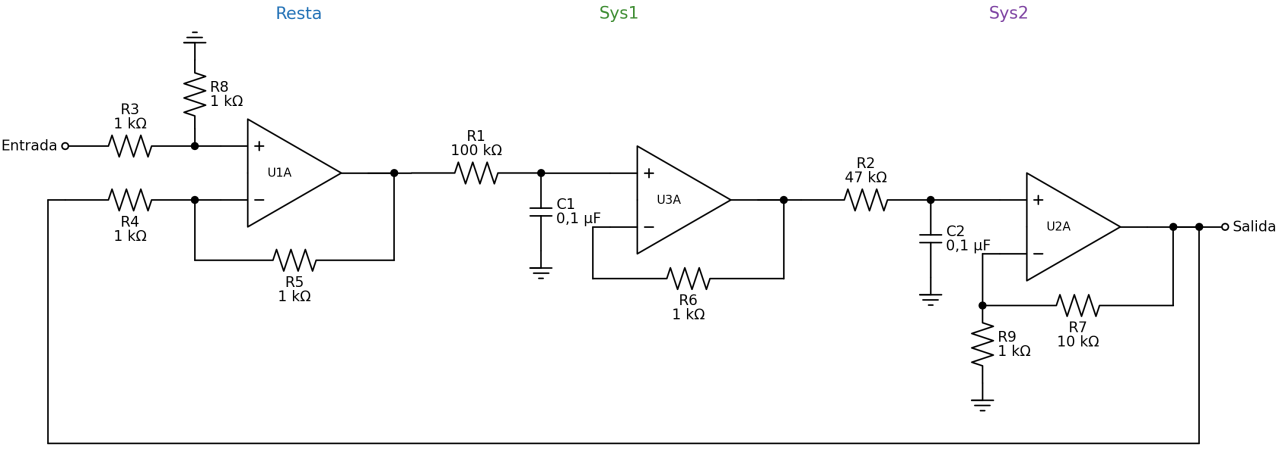
\includegraphics[width=0.85\textwidth]{figuras/figura_1.png}
    \caption{Planta a controlar (alimentación de los operacionales: $\pm 10\text{ V}$).}
    \label{fig:circuito}
\end{figure}

\begin{figure}[H]
    \centering
    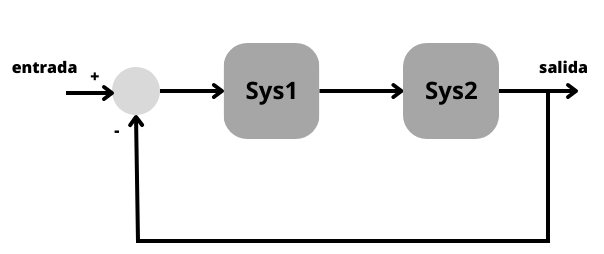
\includegraphics[width=0.5\textwidth]{figuras/figura_2.png}
    \caption{Diagrama de bloques de la planta a controlar.}
    \label{fig:bloques}
\end{figure}

\section{Modelado}

\subsection{Funciones de transferencia por bloques (Fig. 2)}
Considerando amplificadores operacionales ideales en zona lineal ($I_+ = I_- = 0$ y $V_+ = V_-$):

\paragraph{Bloque Resta ($U_{1A}$):}
En el terminal no inversor tenemos un divisor resistivo entre $R_3$ y $R_8$ ($R_3 = R_8 = 1\text{ k}\Omega$):
\begin{equation}
    V_+ = V_{\text{Entrada}} \frac{R_8}{R_3 + R_8} = \frac{1}{2} V_{\text{Entrada}}
\end{equation}
En el nodo inversor, planteando corrientes con $R_4 = R_5 = 1\text{ k}\Omega$:
\begin{equation}
    \frac{V_{\text{Salida}} - V_-}{R_4} + \frac{V_{\text{resta}} - V_-}{R_5} = 0 \implies V_- = \frac{V_{\text{Salida}} + V_{\text{resta}}}{2}
\end{equation}
Igualando $V_+ = V_-$ resulta:
\begin{equation}
    V_{\text{resta}}(s) = V_{\text{Entrada}}(s) - V_{\text{Salida}}(s)
\end{equation}
Por lo tanto, la etapa con $U_{1A}$ implementa el restador unitario de entrada del lazo.

\paragraph{Bloque $\text{Sys}_1$ ($R_1$, $C_1$ y $U_{3A}$):}
La red $R_1 C_1$ forma un divisor de impedancias a la entrada no inversora de $U_{3A}$. Como $I_+ = 0$:
\begin{equation}
    V_{+,U3A}(s) = \frac{\frac{1}{sC_1}}{R_1 + \frac{1}{sC_1}} V_{\text{resta}}(s) = \frac{1}{R_1 C_1 s + 1} V_{\text{resta}}(s)
\end{equation}
El operacional $U_{3A}$ está conectado como seguidor de tensión ($V_{\text{out},U3A} = V_{+,U3A}$), por lo que con $R_1 = 100\text{ k}\Omega$ y $C_1 = 0,1\,\mu\text{F}$ ($\tau_1 = R_1 C_1 = 0,01\text{ s}$):
\begin{equation}
    \text{Sys}_1(s) = \frac{1}{R_1 C_1 s + 1} = \frac{1}{0,01 s + 1}
\end{equation}

\paragraph{Bloque $\text{Sys}_2$ ($R_2$, $C_2$ y $U_{2A}$):}
De manera análoga, la red $R_2 C_2$ en la entrada no inversora de $U_{2A}$ cumple:
\begin{equation}
    V_{+,U2A}(s) = \frac{1}{R_2 C_2 s + 1} V_{\text{out},U3A}(s)
\end{equation}
El operacional $U_{2A}$ está en configuración no inversora con ganancia $k = 1 + \frac{R_7}{R_9}$. Con $R_2 = 47\text{ k}\Omega$, $C_2 = 0,1\,\mu\text{F}$ ($\tau_2 = R_2 C_2 = 0,0047\text{ s}$) y $k = 1 + \frac{10\text{ k}\Omega}{1\text{ k}\Omega} = 11$:
\begin{equation}
    \text{Sys}_2(s) = \frac{k}{R_2 C_2 s + 1} = \frac{k}{0,0047 s + 1}
\end{equation}
Como el seguidor $U_{3A}$ desacopla ambas etapas, el camino directo es el producto $\text{Sys}_1(s) \cdot \text{Sys}_2(s)$ y el circuito queda representado por el diagrama de bloques de la Fig. \ref{fig:bloques}.

\subsection{Función de transferencia en lazo cerrado $\text{Sys}_f(s)$}
Para el lazo con realimentación negativa unitaria, siendo $G(s) = \text{Sys}_1(s)\text{Sys}_2(s)$:
\begin{equation}
    \text{Sys}_f(s) = \frac{\text{Salida}(s)}{\text{Entrada}(s)} = \frac{G(s)}{1 + G(s)} = \frac{k}{(\tau_1 s + 1)(\tau_2 s + 1) + k}
\end{equation}
Desarrollando el denominador y dividiendo por $\tau_1 \tau_2$:
\begin{equation}
    \text{Sys}_f(s) = \frac{\dfrac{k}{\tau_1 \tau_2}}{s^2 + \left(\dfrac{1}{\tau_1} + \dfrac{1}{\tau_2}\right)s + \dfrac{1 + k}{\tau_1 \tau_2}}
\end{equation}
Reemplazando $\tau_1 = 0,01\text{ s}$, $\tau_2 = 0,0047\text{ s}$ y $k = 11$:
\begin{equation}
    \text{Sys}_f(s) = \frac{234042,55}{s^2 + 312,77\,s + 255319,15}
\end{equation}

\subsection{Parámetros $\omega_n$ y $\xi$, e influencia de $k$}
Comparando el denominador con la forma canónica $s^2 + 2\xi\omega_n s + \omega_n^2$:
\begin{align}
    \omega_n &= \sqrt{\frac{1+k}{\tau_1 \tau_2}} = \sqrt{255319,15} \approx 505,29\text{ rad/s} \\
    \xi &= \frac{1/\tau_1 + 1/\tau_2}{2\omega_n} = \frac{312,77}{2 \cdot 505,29} \approx 0,3095
\end{align}
\textbf{Influencia de $k$:} Al aumentar $k$, la frecuencia natural $\omega_n$ aumenta ($\propto \sqrt{1+k}$), haciendo más rápida la respuesta inicial, mientras que el amortiguamiento $\xi$ disminuye ($\propto 1/\sqrt{1+k}$), provocando mayores oscilaciones y un mayor sobrepaso ($PO$). Sin embargo, la atenuación $\sigma = \xi\omega_n = \frac{1}{2}\left(\frac{1}{\tau_1} + \frac{1}{\tau_2}\right) = 156,38\text{ s}^{-1}$ no depende de $k$, por lo que el tiempo de establecimiento $T_s$ se mantiene prácticamente constante. Además, un mayor $k$ acerca la ganancia estacionaria $\frac{k}{1+k}$ a $1$, reduciendo el error permanente.

\subsection{Función de $R_6$ y del seguidor $U_{3A}$}
\begin{itemize}
    \item \textbf{Resistencia $R_6$:} En la práctica los operacionales reales no son perfectamente ideales y tienen pequeñas corrientes internas en sus entradas; $R_6$ se coloca para balancear esas imperfecciones y evitar tensiones de desbalance (\textit{offset}) a la salida. En el análisis teórico, como asumimos un operacional ideal donde no entra corriente ($I_- = 0$), en $R_6$ no hay caída de tensión ($\Delta V_{R_6} = 0$), por lo que $V_- = V_{\text{out},U3A}$ y no afecta la función de transferencia.
    \item \textbf{Seguidor $U_{3A}$ y efecto de suprimirlo:} Su función es aislar ambas etapas (\textit{buffer}). Como tiene impedancia de entrada casi infinita y de salida nula, evita que la segunda red $R_2 C_2$ le robe corriente al capacitor $C_1$ (efecto de carga), permitiendo que la transferencia sea simplemente el producto $\text{Sys}_1(s) \cdot \text{Sys}_2(s)$. Si elimináramos $U_{3A}$ conectando $R_2$ directamente sobre $C_1$, las dos redes interactuarían entre sí y aparecería un término cruzado $R_1 C_2 s$ en el denominador:
    \begin{equation}
        G_{\text{sin buffer}}(s) = \frac{k}{\tau_1 \tau_2 s^2 + (\tau_1 + \tau_2 + R_1 C_2)s + 1}
    \end{equation}
    lo que correría los polos de la planta, volviendo al sistema más lento y cambiando su amortiguamiento.
\end{itemize}

\section{Respuesta al escalón de $\text{Sys}_f$ ($k = 11$)}
Como el sistema es subamortiguado ($\xi = 0,3095 < 1$), su frecuencia amortiguada es $\omega_d = \omega_n\sqrt{1 - \xi^2} \approx 480,48\text{ rad/s}$ y el ángulo de fase es $\beta = \arccos(\xi) \approx 1,256\text{ rad}$. Ante una entrada en escalón unitario ($1\text{ V}$), la respuesta temporal analítica es:
\begin{equation}
    y(t) = y(\infty)\left[1 - \frac{e^{-\xi\omega_n t}}{\sqrt{1 - \xi^2}}\sin(\omega_d t + \beta)\right] = 0,9167\left[1 - 1,0516\,e^{-156,38\,t}\sin(480,48\,t + 1,256)\right]\text{ V}
\end{equation}
Los parámetros principales de desempeño son:
\begin{itemize}
    \item \textbf{Valor en estado estacionario:}
    \begin{equation}
        y(\infty) = \lim_{s \to 0} \text{Sys}_f(s) = \frac{k}{1+k} = \frac{11}{12} \approx 0,9167\text{ V}
    \end{equation}
    \item \textbf{Sobrepaso porcentual ($PO$):}
    \begin{equation}
        PO = 100 \cdot e^{-\frac{\pi\xi}{\sqrt{1-\xi^2}}} \approx 35,97\% \quad \left(y_{\max} = y(\infty)(1 + PO/100) \approx 1,246\text{ V}\right)
    \end{equation}
    \item \textbf{Tiempo de pico ($T_p$):}
    \begin{equation}
        T_p = \frac{\pi}{\omega_d} = \frac{\pi}{480,48} \approx 6,54\text{ ms}
    \end{equation}
    \item \textbf{Tiempo de establecimiento ($T_s$, criterio del $2\%$):}
    \begin{equation}
        T_s \approx \frac{4}{\xi\omega_n} = \frac{4}{156,38} \approx 25,58\text{ ms}
    \end{equation}
    \item \textbf{Tiempo de subida ($t_r$):}
    \begin{equation}
        t_r = \frac{\pi - \beta}{\omega_d} = \frac{\pi - 1,256}{480,48} \approx 3,92\text{ ms}
    \end{equation}
\end{itemize}

\section{Error en estado estacionario}
La transferencia entre la referencia y el error $E(s) = \text{Entrada}(s) - \text{Salida}(s)$ es:
\begin{equation}
    E(s) = \frac{1}{1 + G(s)} R(s), \qquad G(s) = \frac{k}{(0,01 s + 1)(0,0047 s + 1)}
\end{equation}
Como $G(s)$ no posee polos en el origen ($N = 0$), el sistema es de \textbf{Tipo 0}. Aplicando el Teorema del Valor Final ($e_{ss} = \lim_{s \to 0} s E(s)$):

\begin{itemize}
    \item \textbf{Entrada en escalón unitario ($R(s) = 1/s$):}
    \begin{equation}
        K_p = \lim_{s \to 0} G(s) = k = 11 \implies e_{ss,\text{escalón}} = \frac{1}{1 + K_p} = \frac{1}{1 + k} = \frac{1}{12} \approx 0,0833\text{ V}
    \end{equation}
    \item \textbf{Entrada en rampa unitaria ($R(s) = 1/s^2$):}
    \begin{equation}
        K_v = \lim_{s \to 0} s G(s) = 0 \implies e_{ss,\text{rampa}} = \frac{1}{K_v} = \infty
    \end{equation}
    Al no tener un integrador en lazo abierto, el sistema no puede seguir una entrada en rampa y el error crece indefinidamente con el tiempo.
\end{itemize}

\section{Respuesta para distintos valores de $k$ (serie E24)}
Para realizar la ganancia $k = 1 + \frac{R_7}{R_9}$ con resistencias comerciales de la serie E24 en el rango de $1\text{ k}\Omega$ a $100\text{ k}\Omega$, fijamos $R_9 = 1\text{ k}\Omega$ y calculamos $R_7 = (k - 1)R_9$:
\begin{itemize}
    \item \textbf{$k = 1$:} Se reemplaza $R_7$ por un puente directo ($R_7 = 0\,\Omega$) y se puede desconectar $R_9$ ($R_9 \to \infty$), quedando $U_{2A}$ como seguidor de tensión con $k_{\text{ef}} = 1$.
    \item \textbf{$k = 3,2$:} $R_7 = 2,2\text{ k}\Omega$ y $R_9 = 1\text{ k}\Omega \implies k_{\text{ef}} = 1 + \frac{2,2}{1} = 3,2$.
    \item \textbf{$k = 5,7$:} $R_7 = 4,7\text{ k}\Omega$ y $R_9 = 1\text{ k}\Omega \implies k_{\text{ef}} = 1 + \frac{4,7}{1} = 5,7$.
    \item \textbf{$k = 34$:} $R_7 = 33\text{ k}\Omega$ y $R_9 = 1\text{ k}\Omega \implies k_{\text{ef}} = 1 + \frac{33}{1} = 34$.
\end{itemize}
Como $2,2$, $4,7$ y $33$ son valores exactos de la serie E24, en los cuatro casos el $k$ efectivo coincide exactamente con el valor pedido (error relativo del $0\%$). En la Tabla \ref{tab:punto4} se resumen los parámetros calculados con las expresiones de los puntos anteriores.

\begin{table}[H]
    \centering
    \begin{tabular}{c c c c c c c c c}
        \toprule
        \textbf{$k$} & \textbf{$R_7 / R_9$} & \textbf{$\omega_n$ [rad/s]} & \textbf{$\xi$} & \textbf{PO [\%]} & \textbf{$T_p$ [s]} & \textbf{$T_s$ [s]} & \textbf{$y(\infty)$} & \textbf{$e_{ss}$} \\
        \midrule
        $1$ & $0\,\Omega$ / $\infty$ & $206,28$ & $0,7581$ & $2,59$ & $0,0234$ & $0,0256$ & $0,5000$ & $0,5000$ \\
        $3,2$ & $2,2\text{ k}\Omega\,/\,1\text{ k}\Omega$ & $298,93$ & $0,5231$ & $14,54$ & $0,0123$ & $0,0256$ & $0,7619$ & $0,2381$ \\
        $5,7$ & $4,7\text{ k}\Omega\,/\,1\text{ k}\Omega$ & $377,56$ & $0,4142$ & $23,94$ & $0,0091$ & $0,0256$ & $0,8507$ & $0,1493$ \\
        $34$ & $33\text{ k}\Omega\,/\,1\text{ k}\Omega$ & $862,95$ & $0,1812$ & $56,05$ & $0,0037$ & $0,0256$ & $0,9714$ & $0,0286$ \\
        \bottomrule
    \end{tabular}
    \caption{Parámetros teóricos de la respuesta al escalón para los cuatro valores de $k$.}
    \label{tab:punto4}
\end{table}

\end{document}
